\documentclass[10pt,a4paper]{article}
\usepackage[utf8]{inputenc}
\usepackage[english]{babel}
\usepackage{amsmath}
\usepackage{amsfonts}
\usepackage{amssymb}
\usepackage{listings}
\usepackage{graphicx}
\usepackage{hyperref}
\setcounter{tocdepth}{1}
\title{An Alga tutorial}
\date{}

\begin{document}
\maketitle
\tableofcontents
\section{Introduction}

Here you will learn the basis of \href{http://hackage.haskell.org/package/algebraic-graphs}{Alga}, an implementation of an algebra of graphs.
Every given example is runnable, so please feel free to install alga (with \verb|cabal| or \verb|stack|) and have a GHCi console near you if you want to try the code. All you need to have is inside the \verb|Algebra.Graph| module. Don't hesitate to have a look at the \href{http://hackage.haskell.org/package/algebraic-graphs-0.1.1.1/docs/Algebra-Graph.html}{module documentation} if you want more informations.
\\
\\
If you encounter any bug (I hope that you will not), please open an issue at \url{https://github.com/snowleopard/alga/issues/}.

\section{The graph definition}
\subsection{The problem}
Graphs are traditionally defined as a pair comprising a set $V$ of vertices and a set $E \subseteq V \times V$ of edges. This is great when working with traditional imperative languages, but leads to some problems when trying to use it in functional languages such as Haskell.

The idea of alga is to use an other definition of graph, more ``functional-friendly``. And as the most part of the ``functional-friendly” data structures is recursive, such is the alga’s graph definition:

\subsection{A solution}
\begin{lstlisting}[language=Haskell, frame=single]
data Graph a = Empty
             | Vertex a
             | Overlay (Graph a) (Graph a)
             | Connect (Graph a) (Graph a)
\end{lstlisting}

So it says:

\begin{enumerate}
\item You have an only way to construct the empty graph, using the constructor \verb|Empty| which does not take any argument.

\item You can construct a graph from anything, transforming it in a single vertex, using the constructor \verb|Vertex|.

\item You can overlay two graphs, that is just to put them next one to another.

\begin{center}
	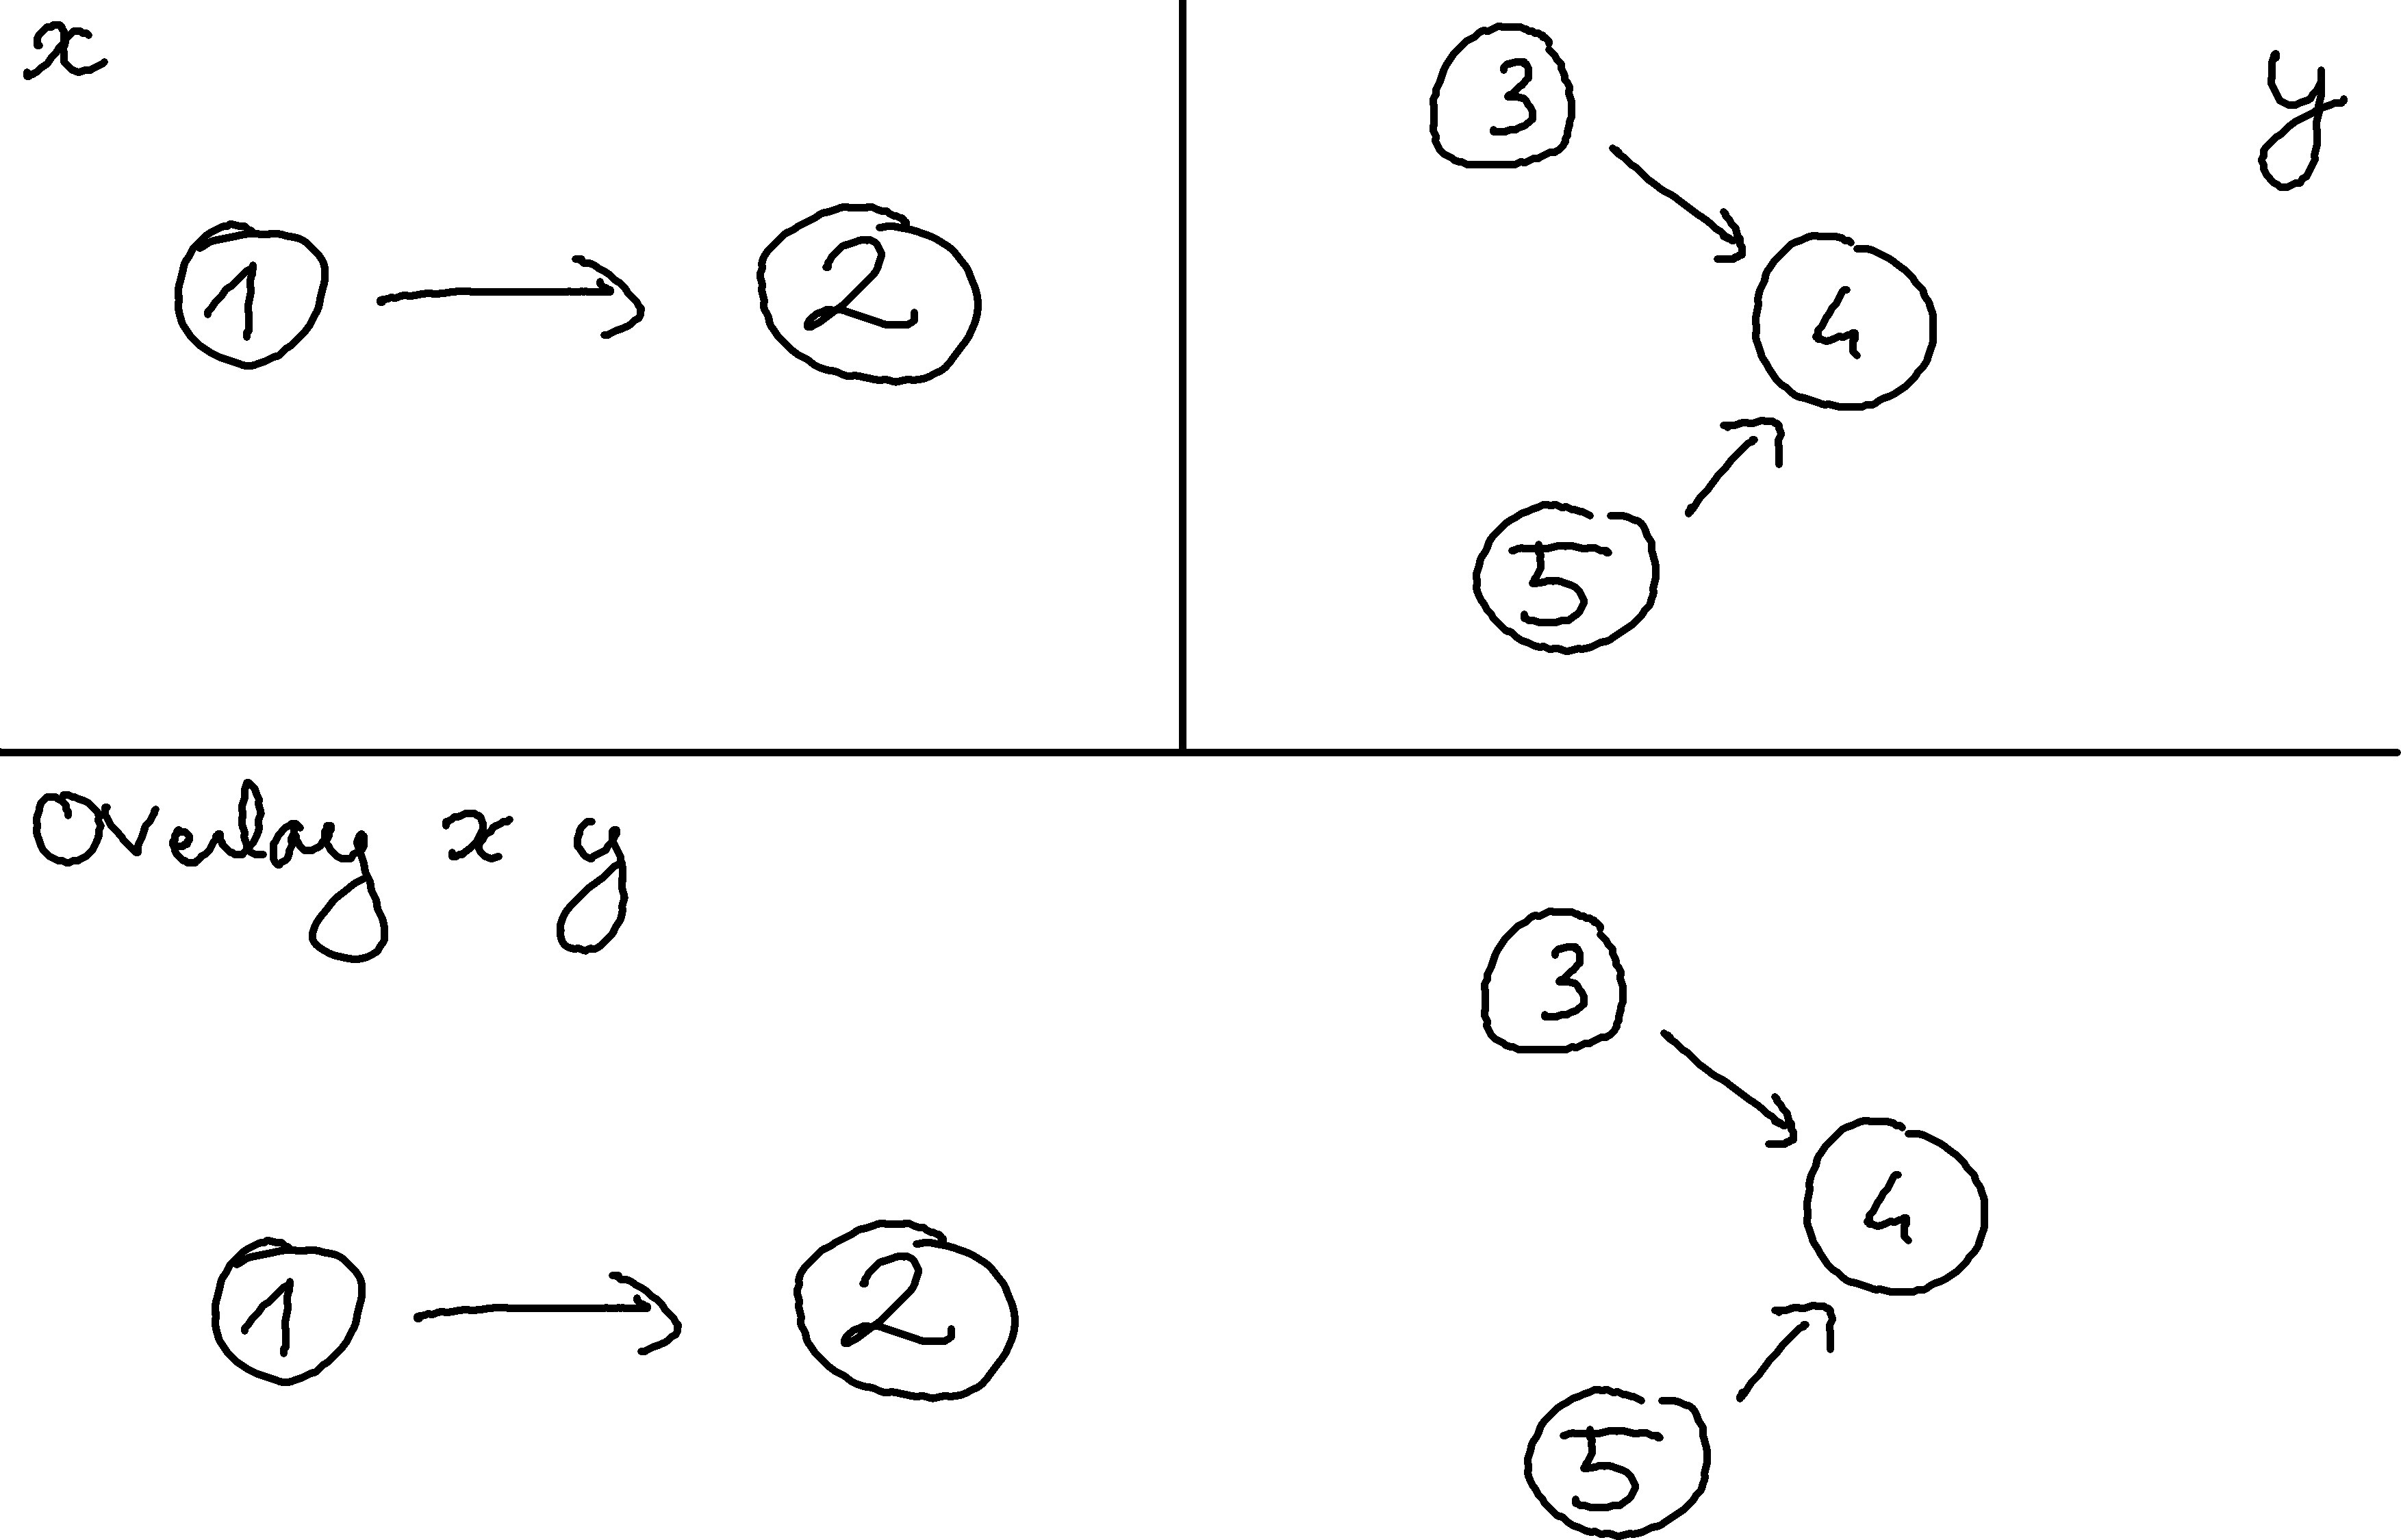
\includegraphics[scale=0.4]{figspng/overlay.png}
\end{center}

\item You can connect two graphs, that is drawing an edge from each vertex of the left side to each vertex to the right side.

\begin{center}
	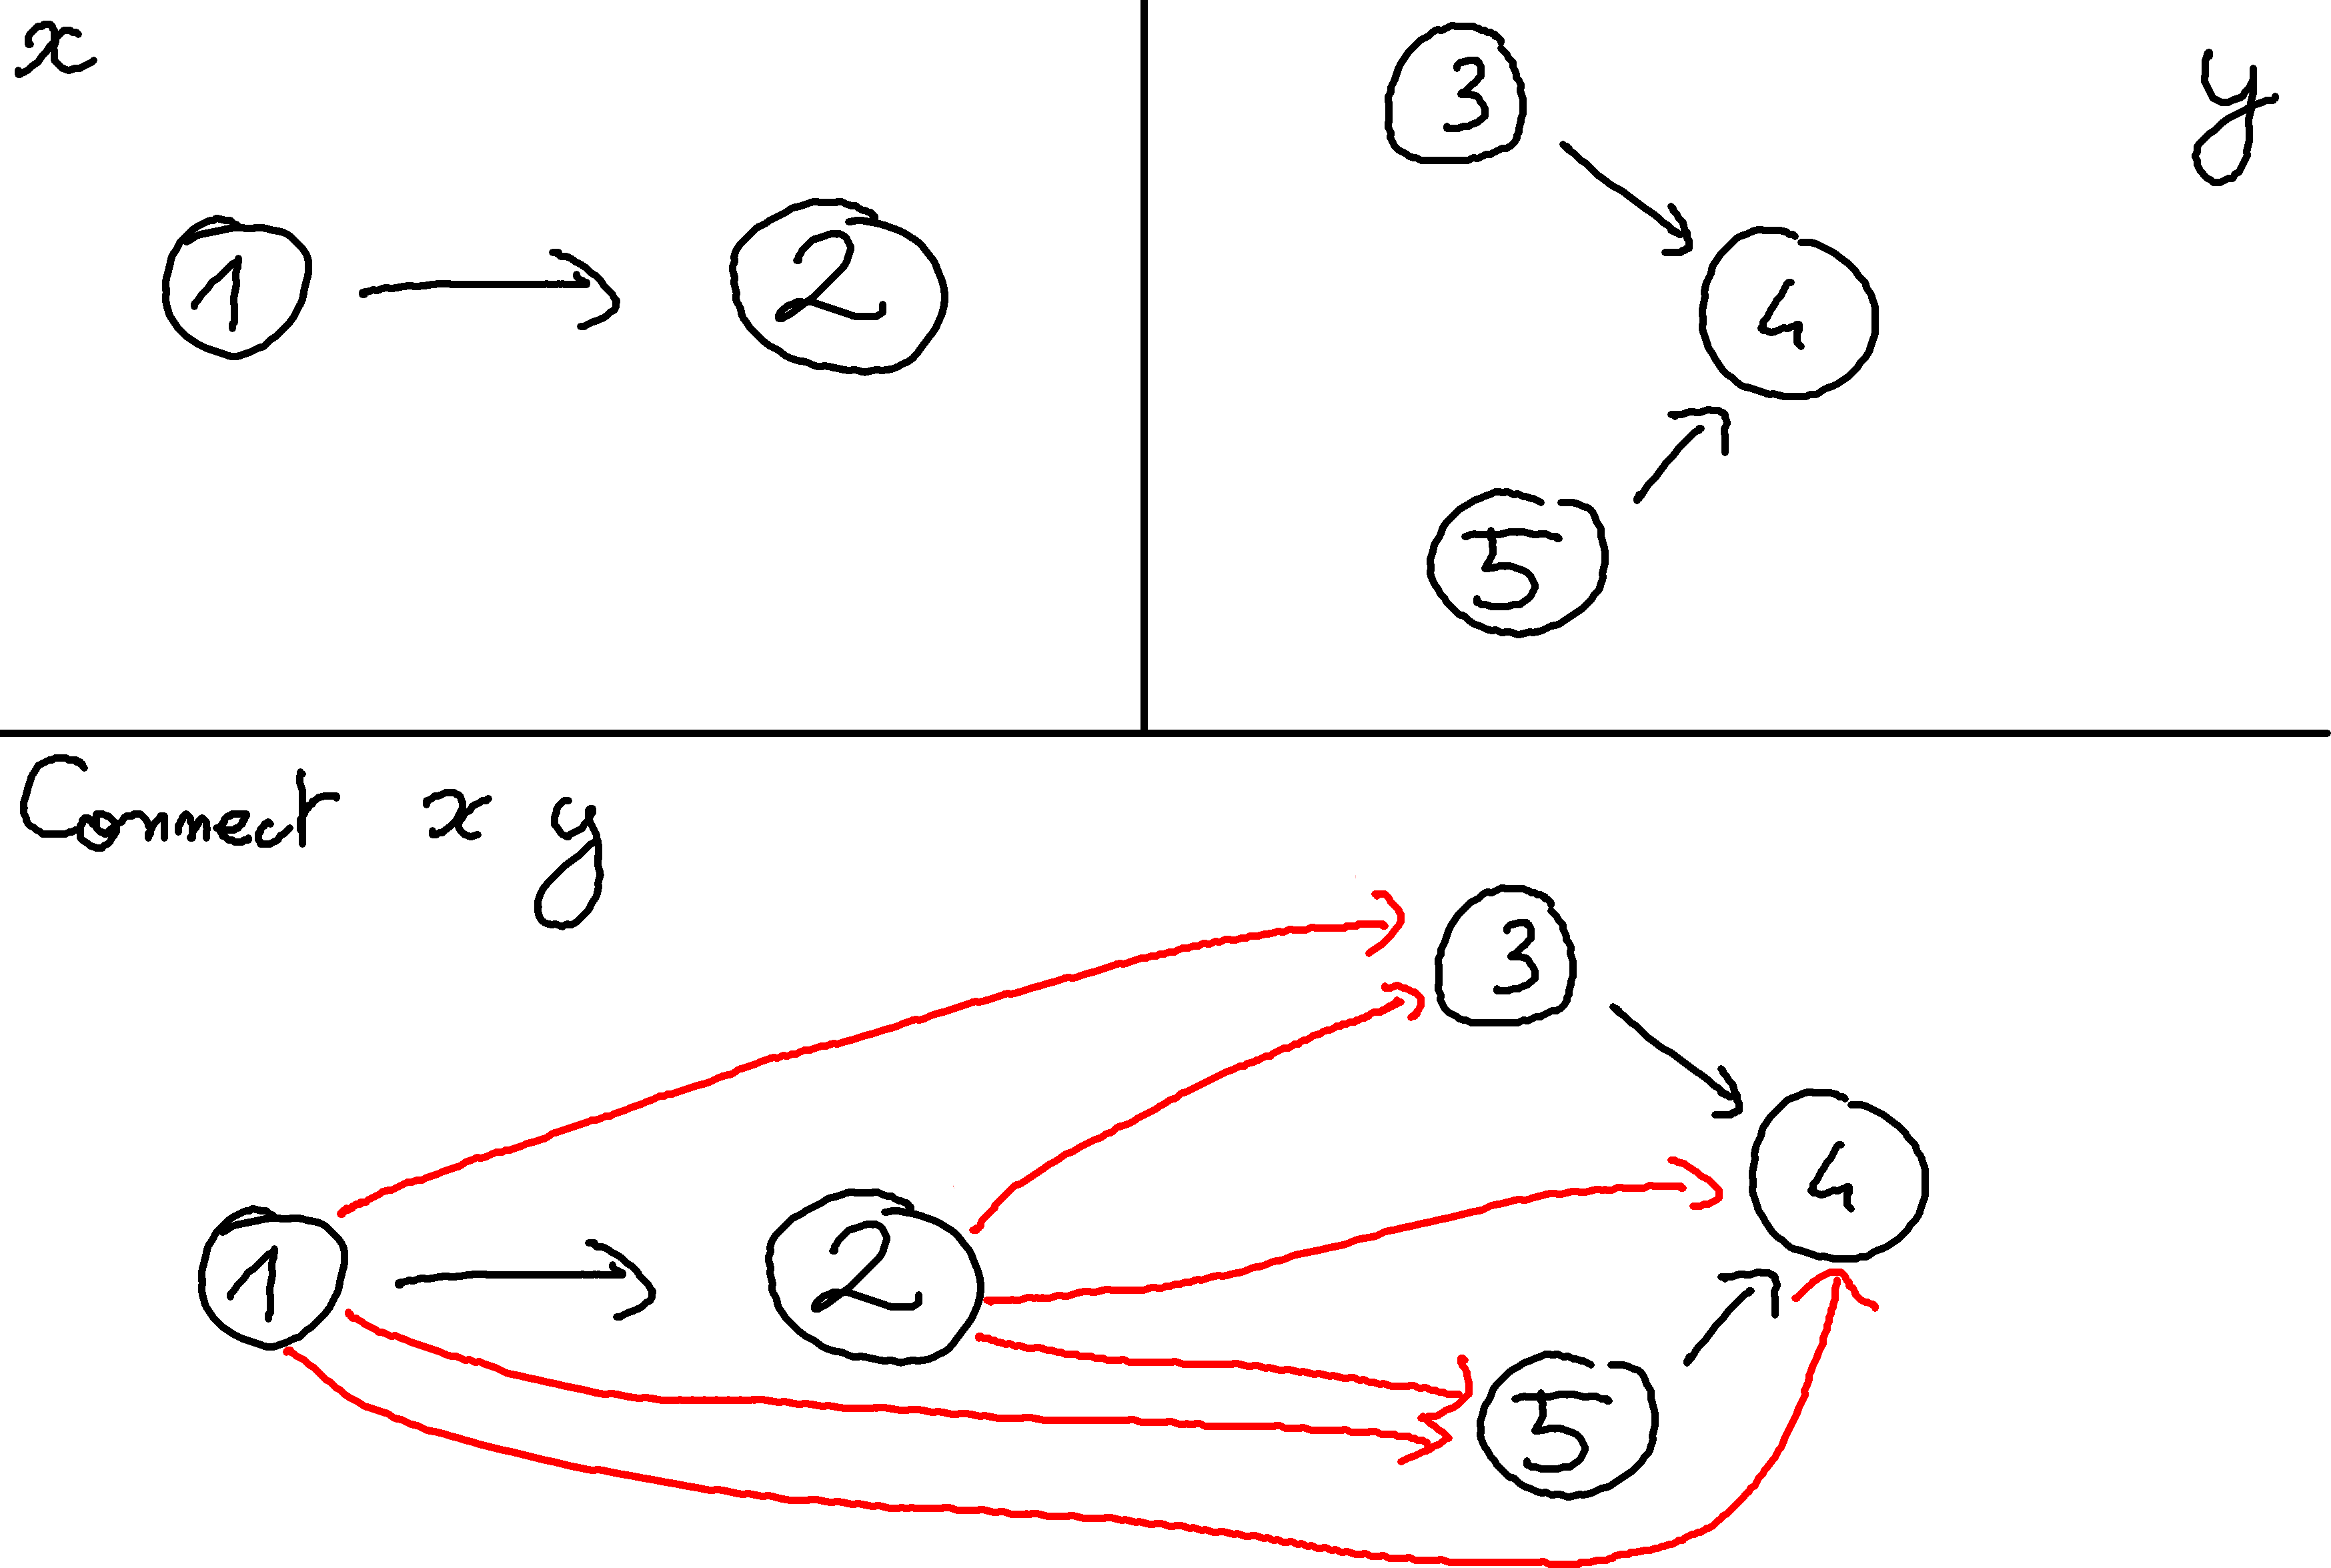
\includegraphics[scale=0.4]{figspng/connect.png}
\end{center}

\end{enumerate}

Simple, no?
\ldots
Well ok this is not a standard way to see a graph, but don't worry, you will get used to it.

Just remember: \emph{The only way to create edges is using} \verb|Connect|.

This definition allow us to deal with \emph{oriented} graphs: An edge from vertex 1 to vertex 2 is NOT the same than an edge from vertex 2 to vertex 1.

\subsection{Some examples}

So, how to use this definition? Here some examples:

\begin{itemize}
	\item A single path, from a vertex 0 to a vertex 1 can be viewed as \verb|Connect (Vertex 0) (Vertex 1)|
	\begin{center}
	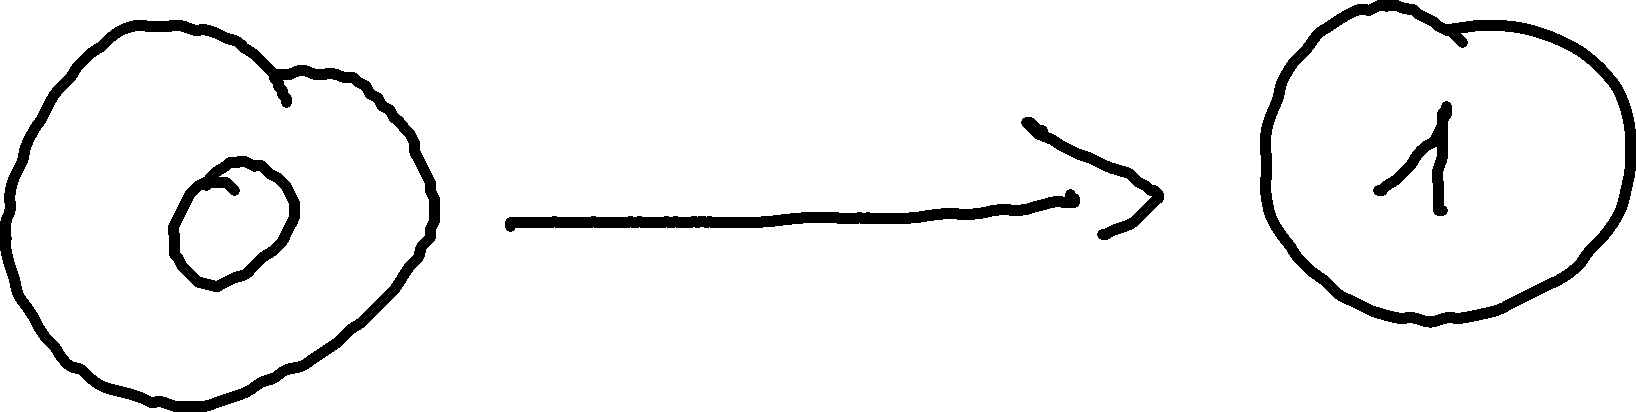
\includegraphics[scale=0.5]{figspng/e2.png}
	\end{center}
	\item A triangle, with an edge from vertex 0 to vertex 1, an edge from vertex 0 to vertex 2, and an edge from vertex 1 to vertex 2 can be viewed as \verb|Connect (Vertex 0) (Connect (Vertex 1) (Vertex 2))|.
	\begin{center}
	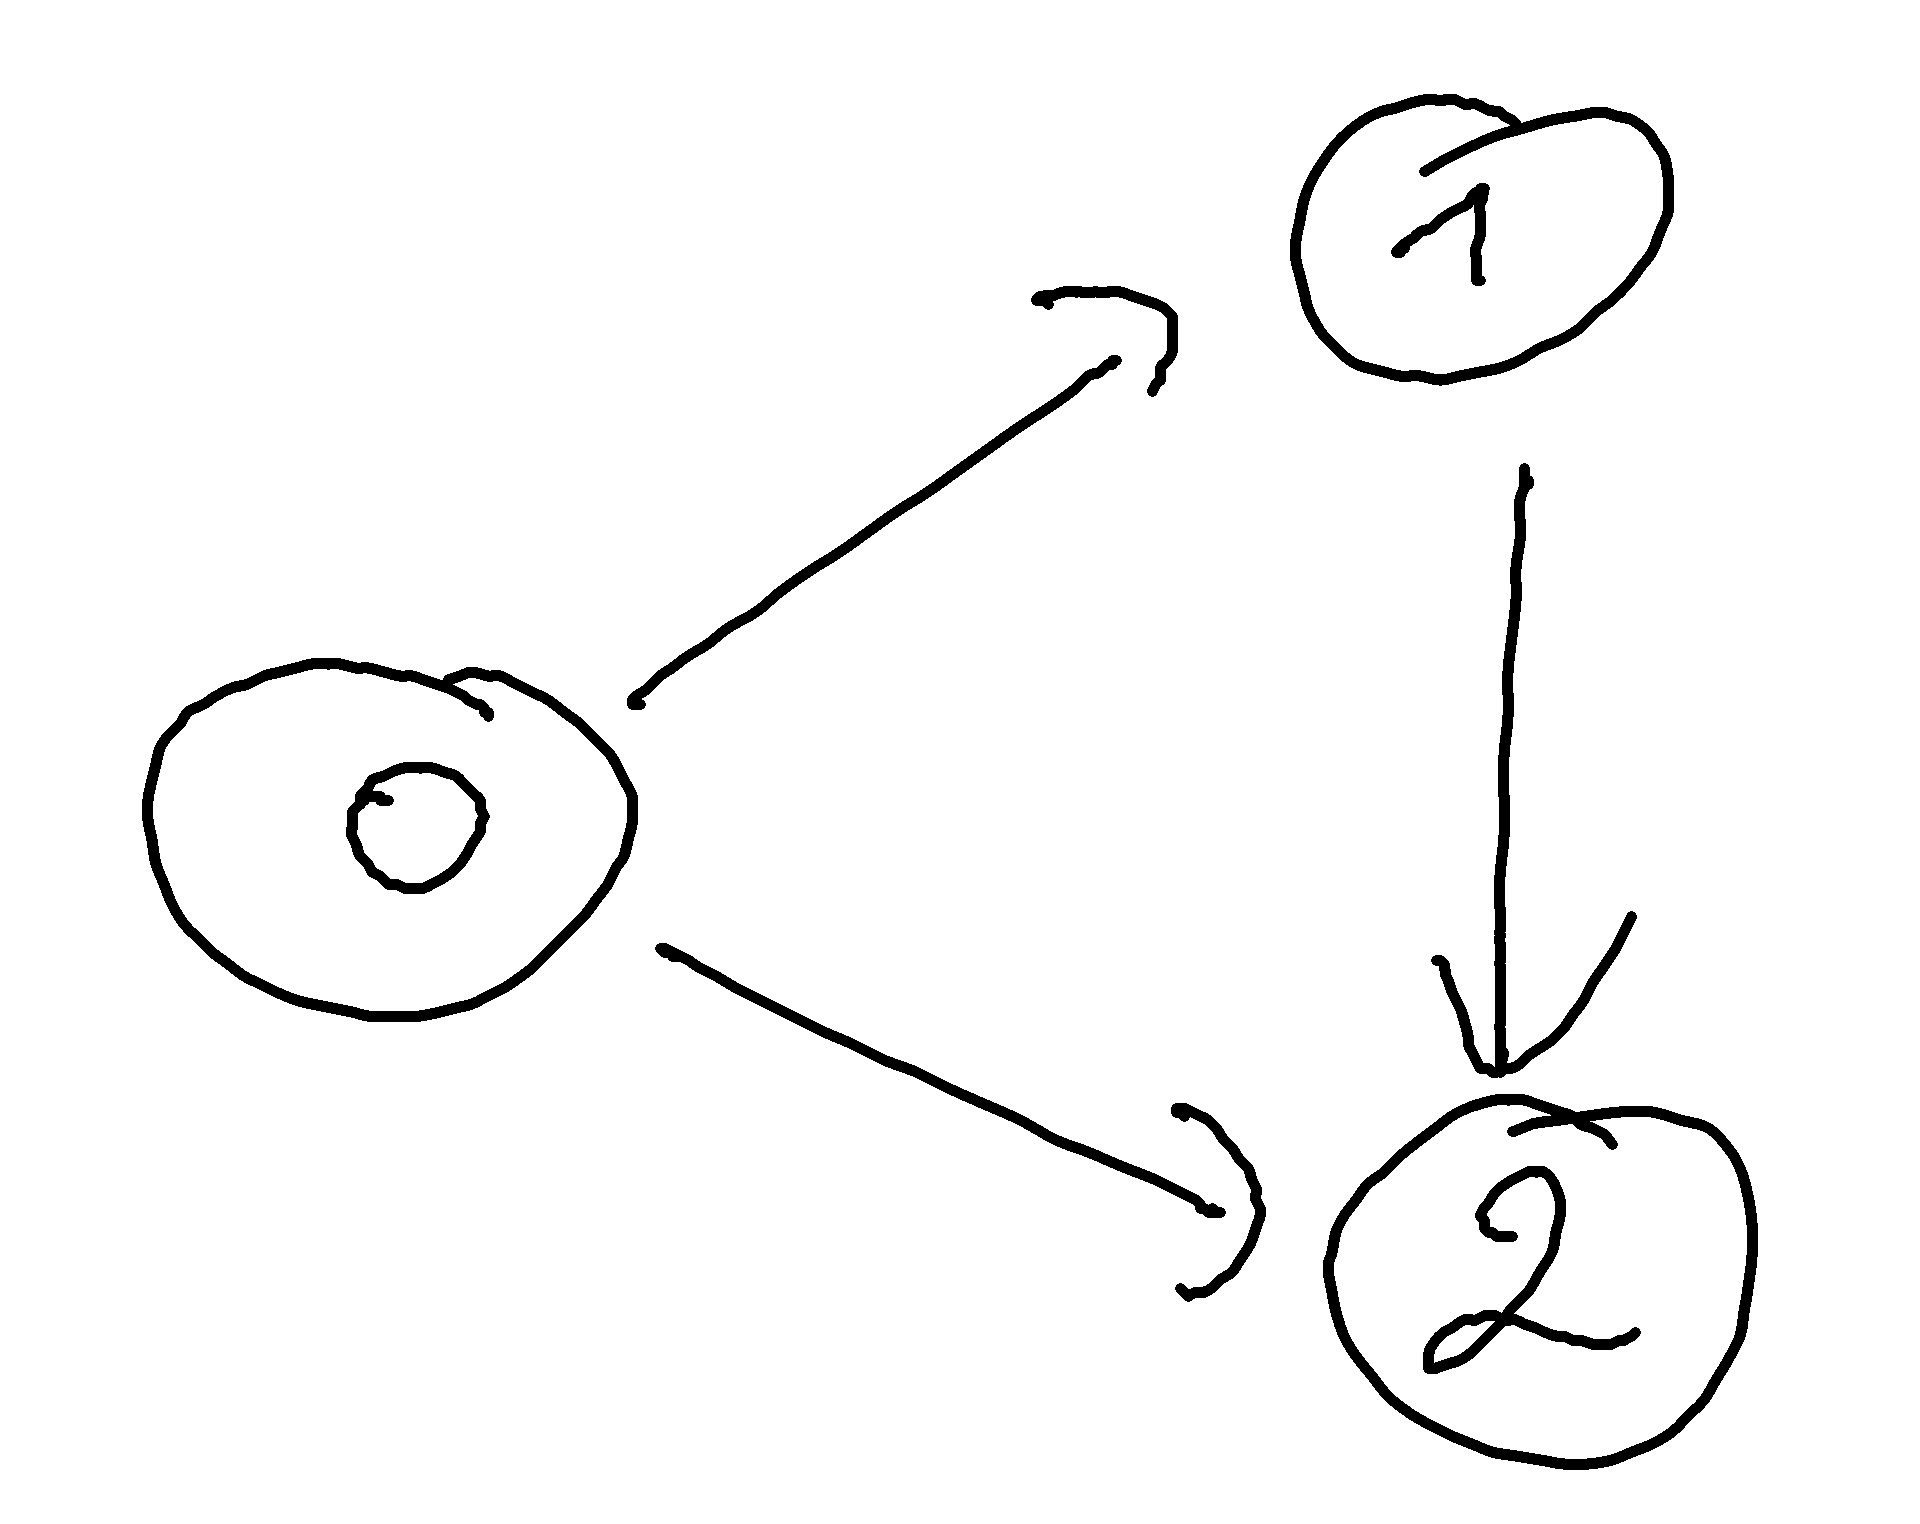
\includegraphics[scale=0.5]{figspng/e1.png}
	\end{center}

\end{itemize}
I heard you from my desktop:
\begin{quote}
	``Berk, but writing big graphs by hand can become very annoying !``
\end{quote}
Don't worry, there are some shortcuts.

\section{Going deeper in the definition}

\subsection{The Num instance}
\verb|Overlay| and \verb|Connect| look like operators, and we want to use them as. So we pose:

\begin{lstlisting}[language=Haskell, frame=single]
(+) = Overlay
(*) = Connect
\end{lstlisting}

In fact, if we have something of the \verb|Num| instance, we can transform it directly into a graph using \verb|Vertex|. This leads to this instance:

\begin{lstlisting}[language=Haskell, frame=single]
instance Num a => Num (Graph a) where
	fromInteger = Vertex . fromInteger
	(+)         = Overlay
	(*)         = Connect
	signum      = const Empty
	abs         = id
	negate      = id
\end{lstlisting}

This means that, in a context of a \verb|Graph|, we have \verb|Vertex 1 == 1|, which is quite useful!

Do you see why alga is an implementation of an \emph{algebra} of graphs? There is a lot of maths here! No please don't run away like you have seen a zombie in a graveyard!  Don't worry, this is not-so-difficult math.

\paragraph{Note}
We will use the \verb|(+)| and \verb|(*)| notation, but these laws are true even when dealing for any graphs.

\subsection{Overlay}

As usual, \verb|(+)| is \emph{associative} (the order in which you are choosing to overlay graphs is not important):
\begin{lstlisting}[language=Haskell, frame=single]
(1 + 2) + 3 == 1 + (2 + 3)
\end{lstlisting}

\verb|(+)| is also \emph{commutative} (overlaying $a$ and $b$ is the same as overlaying $b$ and $a$):
\begin{lstlisting}[language=Haskell, frame=single]
1 + 2 == 2 + 1
\end{lstlisting}

\verb|(+)| has \verb|Empty| as a neutral element (overlaying an Empty graph to another graph is this graph):
\begin{lstlisting}[language=Haskell, frame=single]
1 + Empty == 1 == Empty + 1
\end{lstlisting}

\verb|(+)| is \emph{idempotent} (overlaying a graph with itself is the same graph):
\begin{lstlisting}[language=Haskell, frame=single]
1 + 1 == 1
\end{lstlisting}

\subsection{Connect}
As usual, \verb|(*)| is \emph{associative} (the order in which you are choosing to connect graphs is not important):
\begin{lstlisting}[language=Haskell, frame=single]
(1 * 2) * 3 == 1 * (2 * 3)
\end{lstlisting}

\verb|(*)| is NOT \emph{commutative} (drawing an edge from vertex 1 to vertex 2 is not the same as drawing an edge from vertex 2 to vertex 1):
\begin{lstlisting}[language=Haskell, frame=single]
1 * 2 /= 2 * 1
\end{lstlisting}

\verb|(*)| it has \verb|Empty| as a neutral element (connecting an Empty graph to another graph is this graph):
\begin{lstlisting}[language=Haskell, frame=single]
1 * Empty == 1 == Empty * 1
\end{lstlisting}

\verb|(*)| can saturate (connecting three times the same graph is the same as connecting two times the same graph)
\begin{lstlisting}[language=Haskell, frame=single]
1 * 1 * 1 == 1 * 1
\end{lstlisting}

Why \verb|(*)| is not \emph{idempotent}? Because connecting a vertex with himself allow to create a \emph{loop}:

\begin{center}
	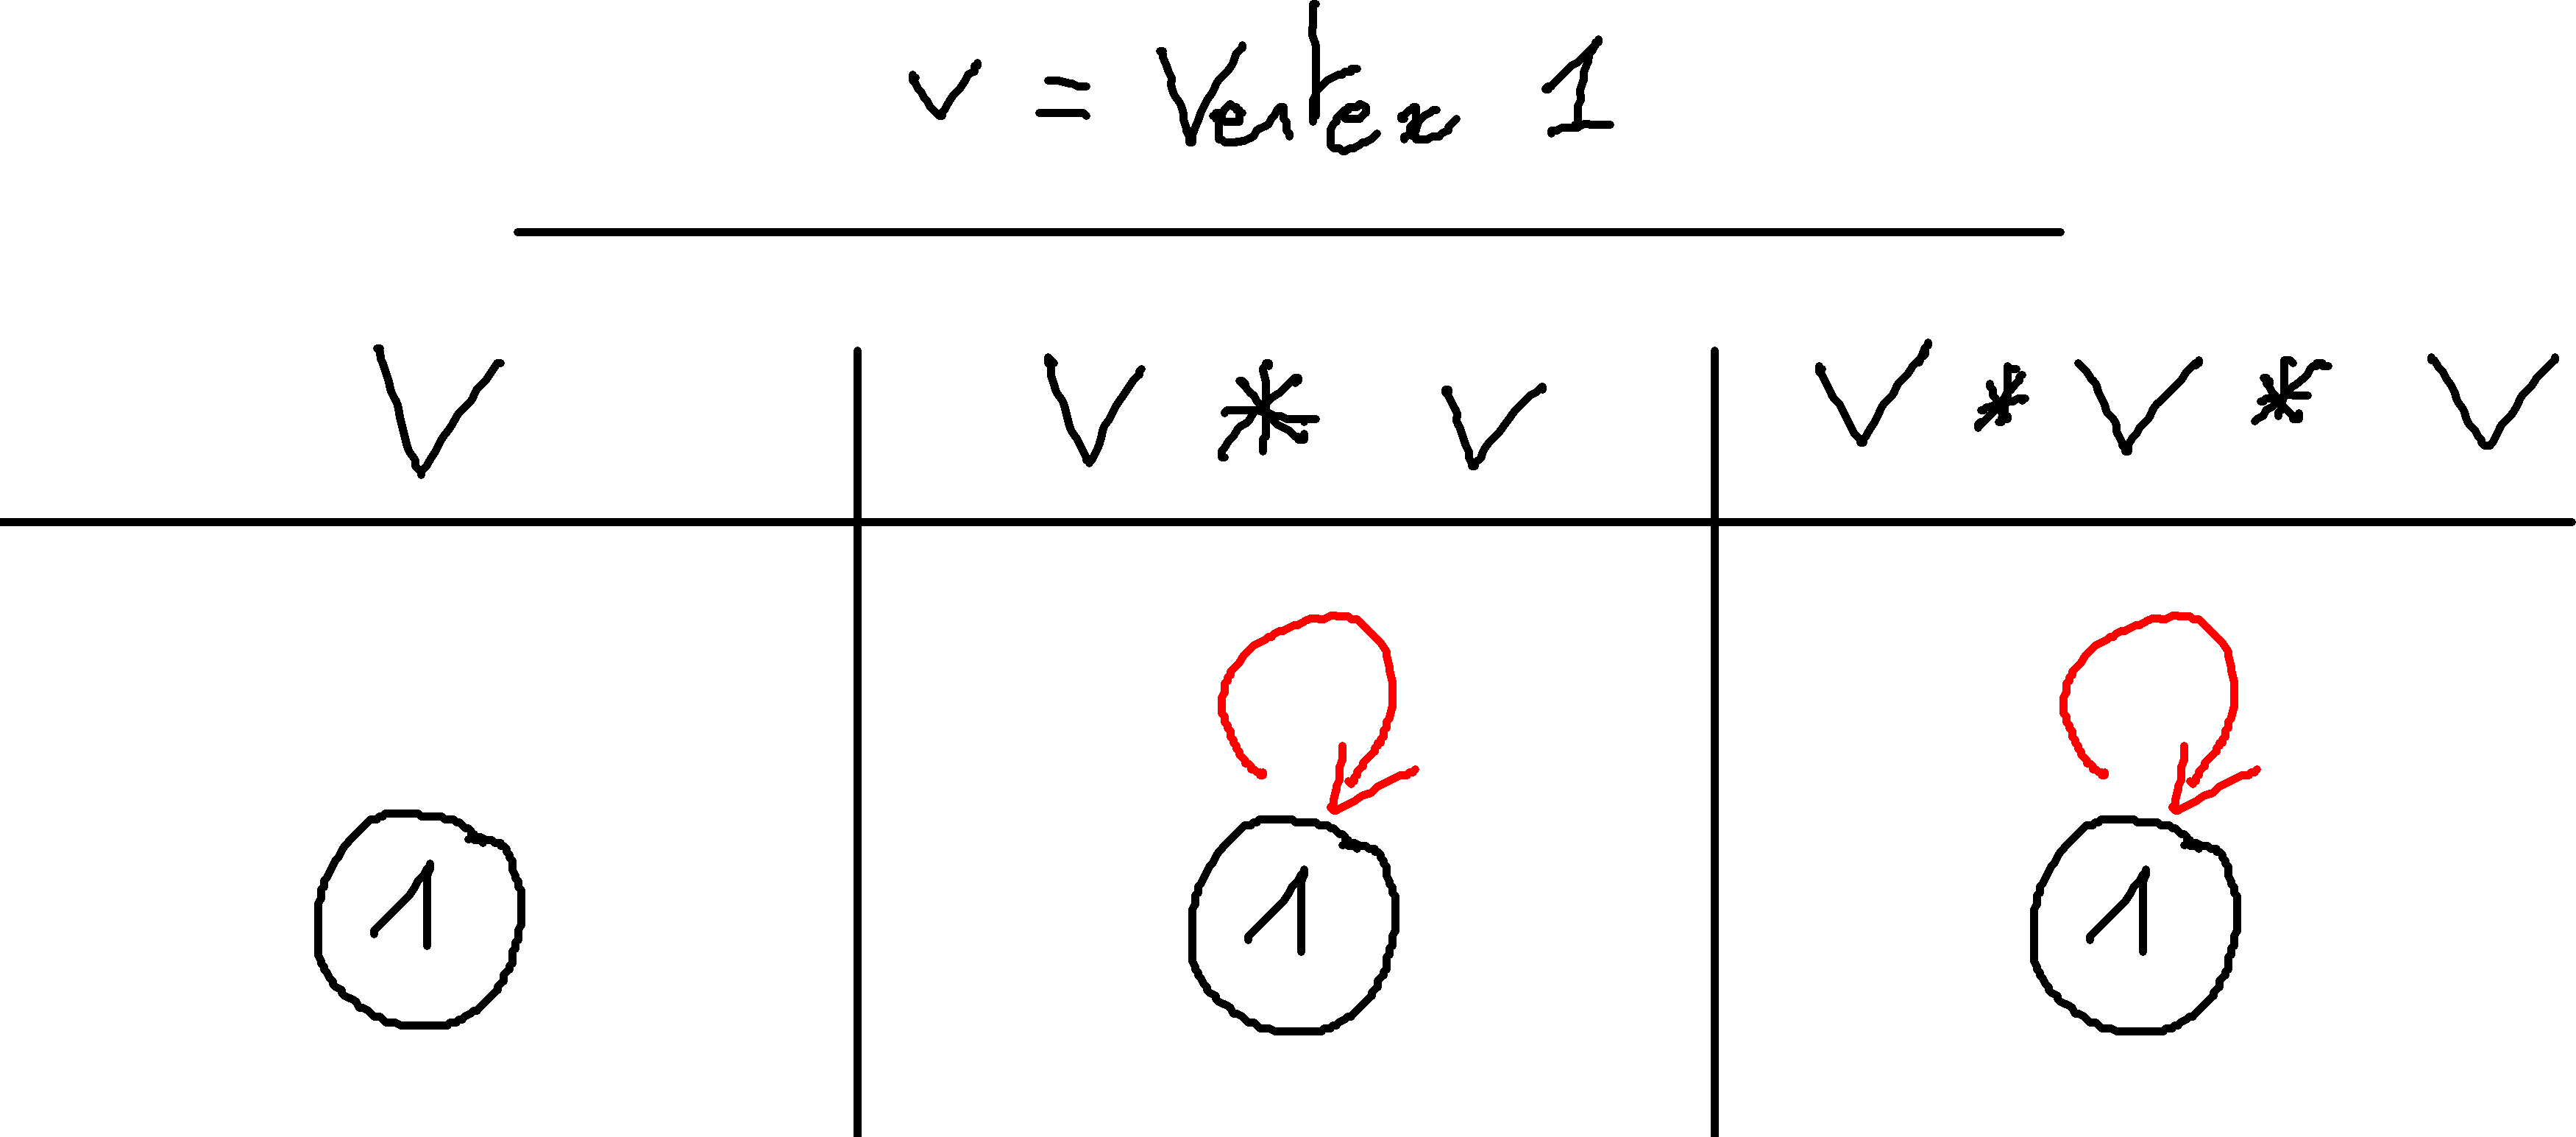
\includegraphics[scale=0.5]{figspng/saturate.png}
\end{center}

\subsection{The two together}
Do you remind when you have discovered that you can mix $+$ and $*$ in the same equation? This is the same thing here!
\begin{lstlisting}[language=Haskell, frame=single]
1 * (2 + 3) == 1 * 2 + 1 * 3
\end{lstlisting}
Here, connecting the single vertex 1 to both 2 and 3 can be done of two \emph{equivalent} ways:
\begin{itemize}
	\item either you are connecting 1 to 2 and 3 ``overlayed``.
	\item or you are overlaying the two edges \verb|(1,2)| and \verb|(1,3)|
\end{itemize}

Whew, this is done we can  make a step forward.

\subsection{Making graphs}
I haven't answered on question yet:
\begin{quote}
	Is the definition usable? Can we represent every graph in alga's representation ?
\end{quote}

Let's try to answer this \emph{important} question. As said, graphs are (almost all the time) defined as a pair $V$ of vertices and $E \subseteq V \times V$ a set of edges. So to prove that we can represents any graph, we need to define a function \verb|create :: [a] -> [(a,a)] -> Graph a| that create a graph from this standard representation.

Ok, let's forget about the edges, we are first going to make \verb|vertices :: [a] -> Graph a| that transform a list of vertices into a \verb|Graph| containing all the single vertices. It looks like we are going to \verb|fold| a list

\begin{lstlisting}[language=Haskell, frame=single]
vertices :: [a] -> Graph a
vertices = foldr (\v g -> Overlay (Vertex v) g) Empty
\end{lstlisting}

Any idea how to do \verb|edges :: [(a,a)] -> Graph a|? The same way, obviously:

\begin{lstlisting}[language=Haskell, frame=single]
edges :: [(a,a)] -> Graph a
edges = foldr
  (\(x,y) g -> Overlay (Connect (Vertex x) (Vertex y)) g)
  Empty
\end{lstlisting}

And so, what can be our \verb|create :: [a] -> [(a,a)] -> Graph a|? Simply:
\begin{lstlisting}[language=Haskell, frame=single]
create :: [a] -> [(a,a)] -> Graph a
create v e = Overlay (vertices v) (edges e)
\end{lstlisting}

So we have defined the desired function, thus we can safely use this definition!

\section{The benefits of the definition}
\subsection{foldg}
On of the very advantage given by this representation is the ability to define the \verb|foldg| function, a kind of adapted \verb|fold| for graph:
\begin{lstlisting}[language=Haskell, frame=single]
foldg :: b -> (a -> b) -> (b -> b -> b)
      -> (b -> b -> b) -> Graph a -> b
foldg e v o c = go
	where
	go Empty         = e
	go (Vertex  x  ) = v x
	go (Overlay x y) = o (go x) (go y)
	go (Connect x y) = c (go x) (go y)
\end{lstlisting}
In other words, the \verb|foldg| function take a base case for \verb|Empty| graphs, something to transform a \verb|Vertex|, and combining functions when we encounter \verb|Overlay| or \verb|Connect|.

\subsection{transpose}

We have a wonderful graph and we want to \verb|transpose| it. Transposing an oriented graph consist in inverting the orientation of all edges. Using \verb|foldg|, this is a piece of cake:

\begin{lstlisting}[language=Haskell, frame=single]
transpose :: Graph a -> Graph a
transpose = foldg Empty Vertex Overlay (flip Connect)
\end{lstlisting}

\subsection{induce}

Still not convinced? Let's try to build an induced sub-graph. An induced sub-graph is a sub-graph that ``forget`` about some vertices and all edges to and from these vertices.

So, we are going to code the \verb|induce :: (a -> bool) -> Graph a -> Graph a| function. We will use \verb|foldg| of course

What is the base case? Do we need to change an \verb|Empty| graph? No of course:

\begin{lstlisting}[language=Haskell, frame=single]
induce :: (a -> Bool) -> Graph a -> Graph a
induce predicate = foldg
  Empty
  undefined
  undefined
  undefined
\end{lstlisting}

Then if we encounter a vertex, we need to verify if it satisfy the predicate. If it does not, we will simply replace it\ldots  Let's say by the empty graph!

\begin{lstlisting}[language=Haskell, frame=single]
induce :: (a -> Bool) -> Graph a -> Graph a
induce predicate = foldg
  Empty
  (\x -> if predicate x then Vertex x else Empty)
  undefined
  undefined
\end{lstlisting}

And finally do we need to touch connection between base graphs? Not at all! Remember, \verb|Empty| is the neutral element of \emph{both} \verb|Connect| and \verb|Overlay|. So we can leave our empty graphs inside the structure without problem (don't worry, the real implementation get rid of these empty leaves). So we come to:

\begin{lstlisting}[language=Haskell, frame=single]
induce :: (a -> Bool) -> Graph a -> Graph a
induce predicate = foldg
  Empty
  (\x -> if predicate x then Vertex x else Empty)
  Overlay
  Connect
\end{lstlisting}

So simple, isn't it?

This even allow us to define:

\begin{lstlisting}[language=Haskell, frame=single]
removeVertex :: a -> Graph a -> Graph a
removeVertex x = induce (/=x)
\end{lstlisting}

\subsection{hasEdge}
\verb|foldg| and \verb|induce| are so cool that a good part of the Alga API is made from them. For example, let's take a look at the \verb|hasEdge| definition:
\begin{lstlisting}[language=Haskell, frame=single]
hasEdge :: Ord a => a -> a -> Graph a -> Graph a
hasEdge u v =
	(Connect (Vertex u) (Vertex v) `isSubgraphOf`) .
	induce (`elem` [u, v])
\end{lstlisting}
To check if a graph contains an edge from $x$ to $y$, you can remove every vertices different of $x$ and $y$, and then check if the edge \emph{alone} is a sub-graph of the induced sub-graph.
Note that \verb|hasEdge| is requiring an \verb|Ord| instance because \verb|isSubgraphOf| is requiring it.

\section{The problems of the definition}
\subsection{Equality}
There is no canonical way to define a graph in alga. For example:
\begin{lstlisting}[language=Haskell, frame=single]
Overlay (Vertex 1) (Vertex 2)
== Overlay (Vertex 2) (Vertex 1)
== Connect Empty (Overlay (Vertex 1) (Vertex 2))
== Overlay
  (Connect (Vertex 1) Empty)
  (Connect Empty (Vertex 2))
\end{lstlisting}

Fortunately, you don't have to bother with the internal definition since the \verb|Eq| instance (which provide \verb|(==)|) take care of this problem for you.

Alga is also providing \verb|(===)| which denote \emph{structural} equality, and thus

\begin{lstlisting}[language=Haskell, frame=single]
Overlay (Vertex 1) (Vertex 2)
===
Overlay (Vertex 2) (Vertex 1)
== False
\end{lstlisting}

\subsection{Take care when defining functions}
Here is a nasty function that you can define:
\begin{lstlisting}[language=Haskell, frame=single]
close : Graph A -> Graph A
close Empty         = Empty
close (Vertex x)    = Vertex x
close (Overlay x y) = Connect x y
close (Connect x y) = Connect x y
\end{lstlisting}

Do you see the problem?
\begin{lstlisting}[language=Haskell, frame=single]
>>> let x = Vertex 0
>>> let y = Overlay (Vertex 0) (Vertex 0)
>>> x == y
True
>>> print (close x)
Vertex 0
>>> print (close y)
(Vertex 0) * (Vertex 0)
>>> close x == close y
False
\end{lstlisting}
For the moment, one can mess the internal structure, and the equality loose its meaning (ie $\forall (f: Graph \ A \to Graph \ B) : g = y \implies f \ g = f \ y$ does NOT hold ).

\section{Useful instances}
Alga's graphs are instance of some classical Haskell classes:

\subsection{Eq, Show}
Of course, you have Graph equality, and you can show a Graph. Alga can also export to the \emph{DOT file format} through the \verb|Algebra.Graph.Export.Dot| module.

\subsection{Functor}
Not so surprisingly, \verb|Graph| is an instance of \verb|Functor|:
\begin{lstlisting}[language=Haskell, frame=single]
instance Functor (Graph a) where
  fmap _ Empty = Empty
  fmap f (Vertex a) = Vertex $ f a
  fmap f (Overlay a b) = Overlay (fmap f a) (fmap f b)
  fmap f (Connect a b) = Connect (fmap f a) (fmap f b)
\end{lstlisting}

This means that if you have something to transform a \verb|a| in a \verb|b| then you can transform a \verb|Graph a| into a \verb|Graph b|. For example:

\begin{center}
	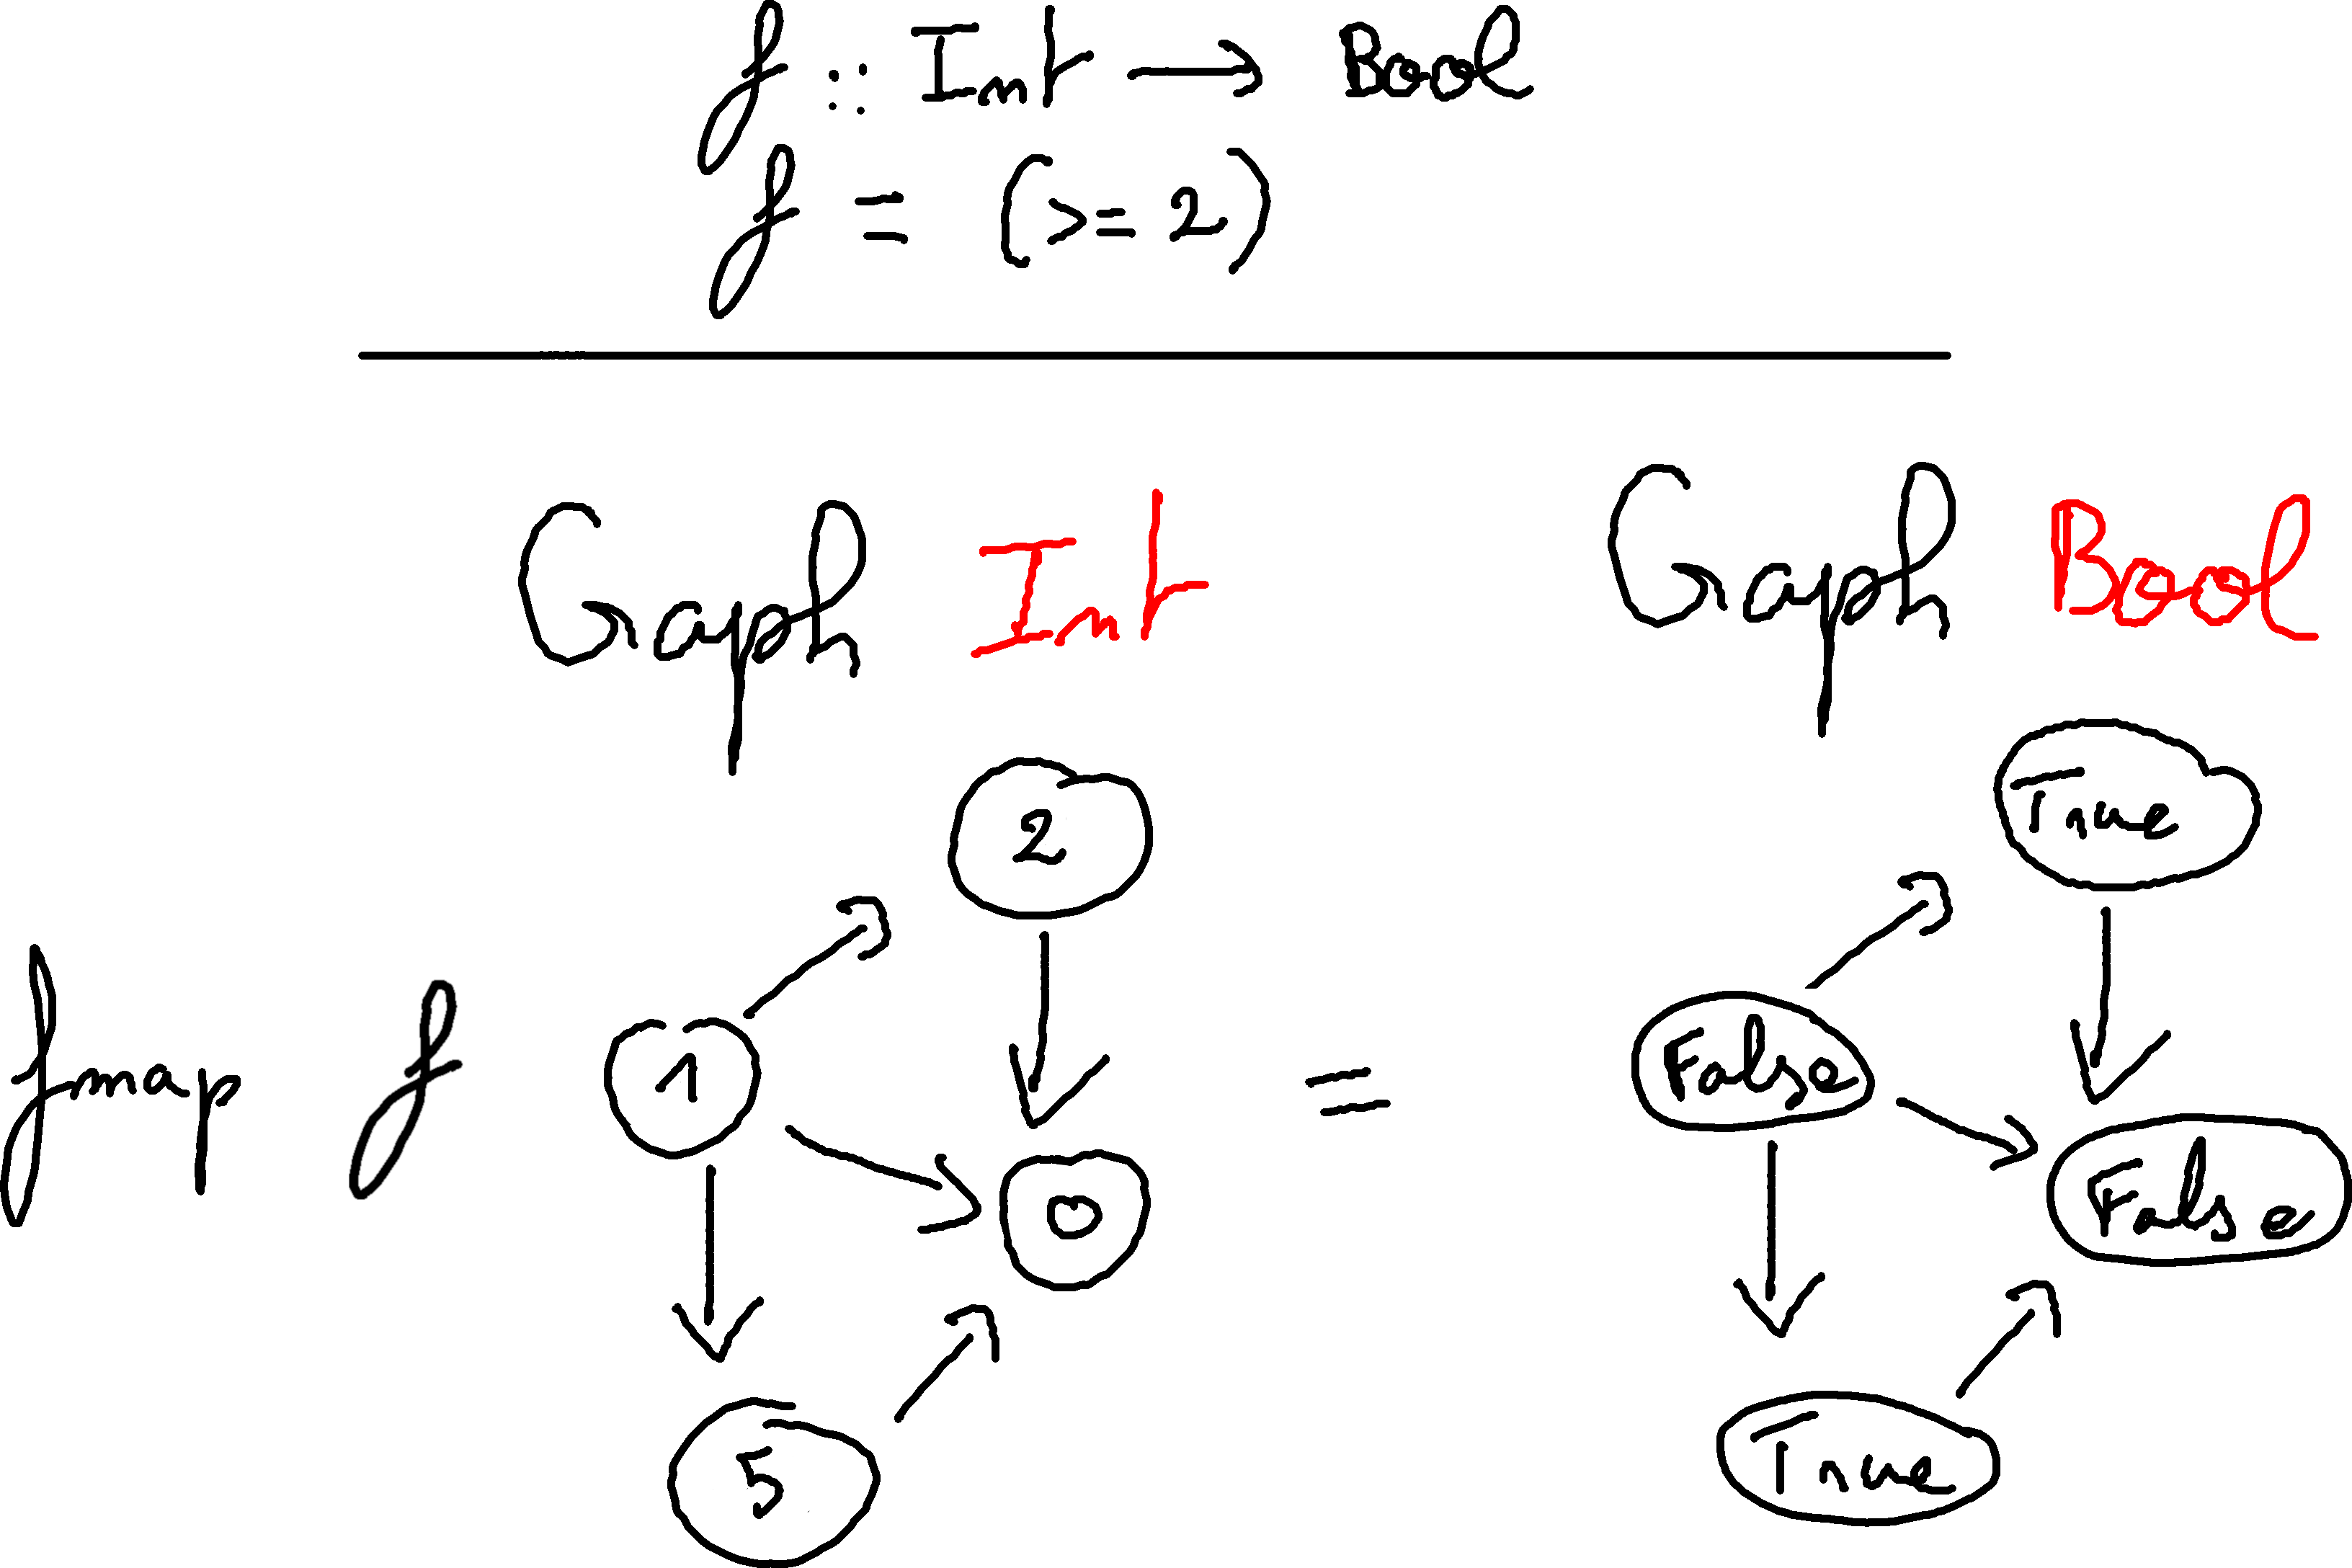
\includegraphics[scale=0.5]{figspng/fmap.png}
\end{center}

If you want to test it, the first graph in alga's representation is: \verb|1 * (2 + 5) * 0|
\\
\\
Alert! Alert! Haskeller's alarms are ringing! If there is a \verb|Functor| instance, is there a \verb|Monad| one?

\subsection{Monad}
\verb|Graph| are indeed a \verb|Monad| instance:
\begin{lstlisting}[language=Haskell, frame=single]
instance Monad (Graph a) where
  return  = Vertex
  g >>= f = foldg Empty f Connect Overlay g
\end{lstlisting}

You can convert anything into a graph, simply by transforming it in a single vertex. Moreover, if you can produce a graph from a type \verb|a| then you can replace every vertex of a \verb|Graph a| with the result, transforming it into a \verb|Graph b|.

For example, one can redefine the previously-viewed \verb|induce| as:

\begin{lstlisting}[language=Haskell, frame=single]
induce :: (a -> Bool) -> Graph a -> Graph a
induce predicate g
  = g >>= (\x -> if predicate x then Vertex x else Empty)
\end{lstlisting}

\subsection{Foldable}
We can in fact define a \verb|Foldable| instance for \verb|Graph|.

This means that you have access to ``lists-like`` functions (like \verb|elem|, \verb|null|). These functions are useful but \emph{not} optimized.

\subsubsection{toList}
It provide also a \verb|toList| function, but WARNING, this is not what you think! It literally transform a graph into a list, so if you had a self-loop or any time two vertices, then you will have two times the same vertex.

In fact, you can use the \verb|Foldable| instance by thinking a graph like a list. For example,

\begin{center}
	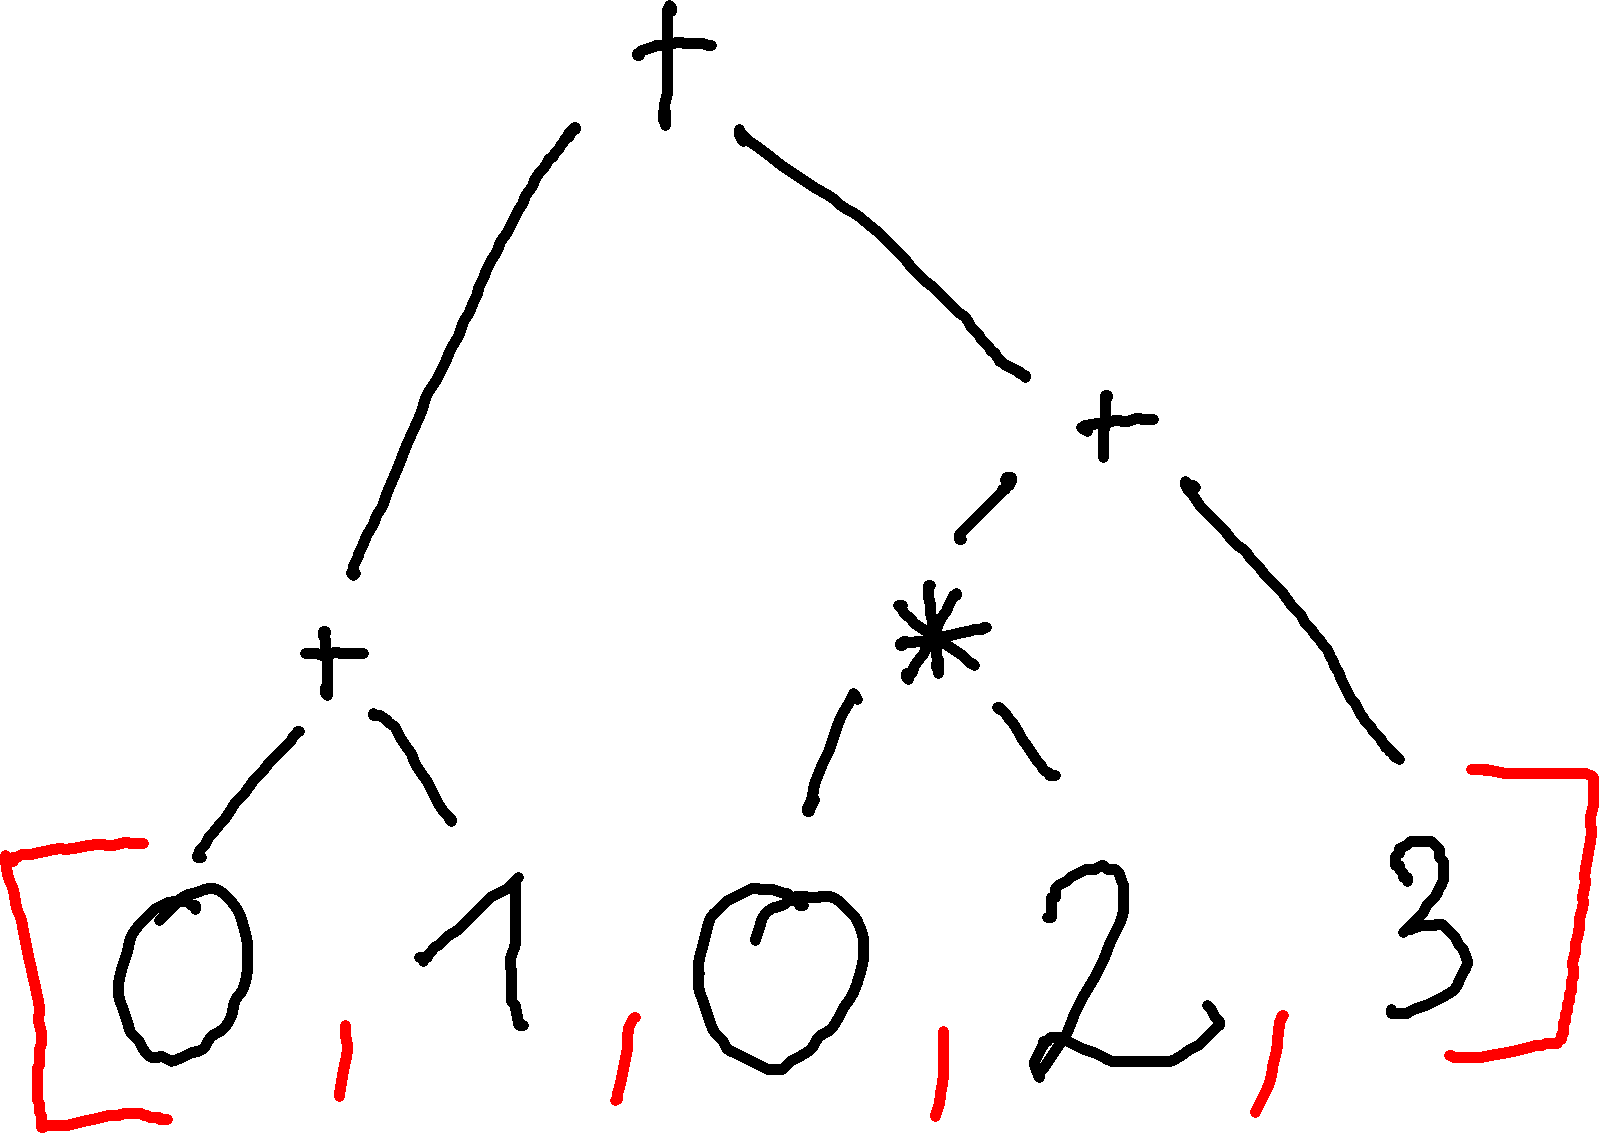
\includegraphics[scale=0.5]{figspng/foldable.png}
\end{center}

\begin{lstlisting}[language=Haskell, frame=single]
toList ((0 + 1) + ((0*2) + 3)) == [0,1,0,2,3]
\end{lstlisting}

Alga is providing a faster \verb|toList| (called \verb|vertexList|) based on \verb|vertexSet| and thus, requiring an \verb|Ord| instance on the vertices. Moreover, \verb|vertexList| give vertices in \emph{ascending order}.
\\
Keep this in mind:
\begin{lstlisting}[language=Haskell, frame=single]
toList /= vertexList
sort . nub . toList == vertexList
\end{lstlisting}

\subsection{Traversable}
More than \verb|Foldable| you have a \verb|Traversable| instance for \verb|Graph|.

Mainly, you can use \verb|sequence :: Monad m => t (m a) -> m (t a)|. Quickly, you can ``strip-out`` a monadic effects. For example, if you have a \verb|Graph (Maybe a)| with leaves set as \verb|Maybe a|, you can have a \verb|Maybe (Graph a)|, set to \verb|Nothing| is there was at least \verb|Nothing| leaf, and \verb|Just gr| if there was \emph{only} \verb|Just| leaves.

\section{An example: A social network}
\subsection{The goal}

Ok, now we are wanting to build something real with all of this. Let's say a social network: one can represent them easily through graphs.
The marketing team analysed the market, and decided to make something ``à la Twitter``. The vertices will be users, and an edge from $x$ to $y$ will denote that $x$ is following $y$.

\subsection{handleRequest}
The staff meeting has chose you to build the \verb|handleRequest| function:
\begin{lstlisting}[language=Haskell, frame=single]
type User = Int

data RequestM = AddUser User
			  | RemoveUser User
			  | ConnectU User User
			  | DisconnectU User User

handleRequestM :: RequestM -> Graph User -> Graph User
\end{lstlisting}

Ok this is now a pretty simple job and the implementation is straightforward:
\begin{lstlisting}[language=Haskell, frame=single]
handleRequestM :: RequestM -> Graph User -> Graph User
handleRequestM (AddUser a) = Overlay (Vertex a)
handleRequestM (RemoveUser a) = removeVertex a
handleRequestM (ConnectU a b) =
	Overlay (Connect (Vertex a) (Vertex b))
handleRequestM (DisconnectU a b) = removeEdge a b
\end{lstlisting}

\subsection{Space is important}
Your company is looking to have many users, so maybe the \verb|ConnectU| is not very wise. In fact, adding a \verb|(Connect (Vertex a) (Vertex b))| is not very alga-friendly. If \verb|a| is connected to 100 people, then \verb|Vertex a| will be 100 times in the representation!
\\
On the advice of your superior, you can change it to:
\begin{lstlisting}[language=Haskell, frame=single]
handleRequestM (ConnectU a b) =
  (>>=) (\x -> if x == a
    then Connect (Vertex x) (Vertex b)
    else Vertex x )
\end{lstlisting}
The modified function will take longer to add a connection (\verb|foldg| has a complexity of $O(n)$), but you will ensure that your graph will not grow too fast (if and only if there is not multiple \verb|Vertex a| hidden in the representation).

\subsection{Inspection}
Viewing that you implemented your function very quickly, you are being asked to help one of your co-workers on his function. He was working about the \verb|getFollowing :: User -> Graph User -> [User]| function.

One possible way is to use the \verb|edgeList :: Ord a => Graph a -> [(a,a)]| function.

\begin{lstlisting}[language=Haskell, frame=single]
getFollowing :: User -> Graph User -> [User]
getFollowing u =
  map snd . filter (\(v,_) -> u == v ) . edgeList
\end{lstlisting}

you can even implement blindly the \verb|getFollowers| function:
\begin{lstlisting}[language=Haskell, frame=single]
getFollowers :: User -> Graph User -> [User]
getFollowers u =
  map fst . filter (\(_,v) -> u == v ) . edgeList
\end{lstlisting}

\subsection{Going IO}
Ok, pure \verb|Graph| inspection is cool, but how do inspect with IO? Your superior want to know from time to time how many users are connected. He has wrote \verb|isConnected| \verb|:: User -> IO Bool|, and he is asking you to write \verb|numberOfConnected| \verb|:: Graph User -> IO Int|. Using \verb|traverse| on the list of the vertices, you quickly answer:
\begin{lstlisting}[language=Haskell, frame=single]
numberOfConnected :: Graph User -> IO Int
numberOfConnected = fmap (length . filter id) .
  traverse isConnected .
  vertexList
\end{lstlisting}

Note that this version is easy to understand and to write, but nor very efficient. One can write a more efficient one using \verb|foldg| and \verb|IntSet|:
\begin{lstlisting}[language=Haskell, frame=single]
import qualified Data.IntSet as Set
import Control.Applicative (liftA2)

numberOfConnected :: Graph User -> IO Int
numberOfConnected = fmap Set.size . foldg
  (return Set.empty)
  (\x -> fmap
    (\y -> if y
       then Set.singleton x
       else Set.empty
    )
    (isConnected x)
  )
  (liftA2 Set.union)
  (liftA2 Set.union)
\end{lstlisting}

\end{document}
